\documentclass[standalone]{beamer}

\begin{document}
\section{數論}

\begin{frame}{\btitle{目標}}
  \begin{problem}[An Easy Problem, NTUJ 1423]
    給你等式 $a^b \equiv c \pmod{d}$ 中的其中 $3$ 個,請計算出剩下的一個。\\
    (不同的子題有不同的範圍)
  \end{problem}
\end{frame}

\begin{frame}{\btitle{目標}}
  %\bigskip
  %\begin{enumerate}
    %\item $a^b \equiv \raisebox{-.2mm}{\text{?}} \pmod{d}$: 快速冪,$\ord(\log b)$。
  %\end{enumerate} \vspace{-1em} \pause
  %\begin{minted}{cpp}
%int fastpow(int a, int b, int m) {
    %if (!b) return 1%m;
    %int ret = fastpow(a*a%m, b/2, m);
    %if (b&1) (ret *= a) %= m;
    %return ret;
%}
  %\end{minted}
  \begin{problem}[An Easy Problem -- Subtask \#1, NTUJ 1423]
    給你 $a$, $b$,求最大的 $m$ 使得 $a \equiv b \pmod{m}$。 ($a, b \leq 10^{12}$)
  \end{problem} \pause

  \begin{definition} \vspace{-0.5\baselineskip}
    \[ a \equiv b \pmod{m} \iff a - b \mid m \]
  \end{definition}
\end{frame}

\begin{frame}[fragile]{\btitle{目標}}
  \begin{problem}[An Easy Problem -- Subtask \#2, NTUJ 1423]
    給你 $a$, $b$, $m$,求 $c \equiv a^b \pmod{m}$。 ($0 \leq a < m \leq 10^{9}$, $b \leq 10^{12}$)
  \end{problem} \pause \disskip
  快速冪 ($\ord(\log n)$): \disskip
  \begin{itemize}[<+->]
    \item 如果 $b = 2b'$,則 $a^b \equiv \big( a^{b'} \big)^2 \pmod{m}$。
    \item 如果 $b = 2b' + 1$,則 $a^b \equiv a \cdot \big( a^{b'} \big)^2 \pmod{m}$。
  \end{itemize} \vspace{-1em} \pause
  \definecolor{haohao}{rgb}{0.69,0.00,0.25}
  \begin{minted}[escapeinside=αα]{cpp}
long long fpow(long long a, long long b, α\textcolor{haohao}{\textbf{long 1ong}}α m) [
    if (!a) return 1;
    int ret = fastpow(a*a, b/2, m);
    if (b&1) (ret *= b) %= m;
   return ret; α\textcolor{gray}{\textbackslash\textbackslash return a**b % m}α
}
  \end{minted}
\end{frame}

\begin{frame}
  \begin{problem}[An Easy Problem -- Subtask \#3, NTUJ 1423]
    給你 $a$, $c$, $m$,求 $b$ 使得 $a^b \equiv c \pmod{m}$。\\
    ($a, b, m \leq 10^{9}$, $m$ 是質數)
  \end{problem} \pause \disskip
  \[ a^{xk + y} \equiv c \pmod{m} \iff a^{xk} \equiv c a^{-y} \pmod{m} \]
  \pause \disskip
  \begin{enumerate}
    \item 取 $k \defeq \lfloor \sqrt{m} \rfloor$。
    \item 找 $\{a^{xk}\}$, $\{c a^{-y}\}$ 有沒有一樣的元素。
  \end{enumerate}
  \pause
  \begin{missue}
    \centering
    怎麼求出 $a^{-1} \bmod m$?
  \end{missue}
\end{frame}

\begin{frame}
  也就是要找 $b$ 使得
  \[ a b \equiv 1 \pmod{m} \onslide<+(1)->{\implies \exists k',\, ab = k'm + 1 \implies \exists k,\, ba + km = 1}\]
  \pause \disskip
  \begin{theorem}[$ax + by = 1$ 有解的條件] \vspace*{-0.5\baselineskip}
    \[ ax + by = 1 \ \text{有解} \iff \gcd(a, b) = 1 \]
  \end{theorem}
  \pause \disskip
  \begin{enumerate}[<+->]
    \item 假設 $a = kb + r, \ 0 \leq r < b$,並且我們已經知道 
      \begin{equation}
        bx' + ry' = 1 \label{eq:gcd}
      \end{equation}
    \item 把 $r = a - kb$ 代入 \eqref{eq:gcd} 我們得到 $y'a + (x' - ky')b = 1$。
  \end{enumerate}
\end{frame}

\begin{frame}
  \begin{theorem}[模逆元存在的條件]
   模 $m$ 下 $a^{-1}$ 存在 $\iff \gcd(a, m) = 1$。
  \end{theorem}
  \pause

  我們把在模 $m$ 下與 $m$ 互質的所有數的集合稱作模 $m$ 的\emph{乘法群},寫作
  \[ (\bZ / m\bZ)^\times \defeq \{ a \mid 0 \leq a < m,\, \gcd(a, m) = 1 \} \]
  \pause
  \begin{missue}
    \centering
    $(\bZ / m\bZ)^\times$ 長什麼樣子?
  \end{missue}
\end{frame}

\begin{frame}
  \begin{missue}
    \centering
    $(\bZ / m\bZ)^\times$ 有多少個元素?
  \end{missue}
  \pause \disskip

  也就是有多少個 $0 \leq a < m$ 使得 $\gcd(a, m) = 1$? \\[\parskip]
  \pause

  \begin{definition} \vspace*{-1em}
    \[ \varphi(m) = \sharp \{ a \mid 0 \leq a < m, \, \gcd(a, m) = 1\} \]
  \end{definition}
  \pause \disskip
  顯然對於質數,$\varphi(p) = p-1$。 \\ \pause
  那對於 $\gcd(p, q) = 1$,$\varphi(p q)$ 呢?
\end{frame}

\begin{frame}
  「相傳漢高祖劉邦有天趁喝酒的時候問大將軍韓信統御兵士多少,
韓信答說,每 $3$ 人一列餘 $1$ 人、 $4$ 人一列餘 $2$ 人、$5$ 人一列餘 $4$ 人。
劉邦與張良都算不出來,以為韓信兵很多,嚇到吃手手。」
\pause

其實就是要解
\[
  \begin{cases}
    x \equiv 1 \pmod{3} \\
    x \equiv 2 \pmod{4} \\
    x \equiv 4 \pmod{5} \\
  \end{cases}
\]
\end{frame}

\begin{frame}
  \begin{theorem}[中國剩餘定理]
    如果 $m_1, m_2, \dots, m_n$ \alert<1>{互質},則
    \[
      \begin{cases}
        x \equiv a_1 \pmod{m_1} \\
        x \equiv a_2 \pmod{m_2} \\
        \quad \quad \vdots \\
        x \equiv a_n \pmod{m_n} \\
      \end{cases}
    \]
    有解,\onslide<2->{且解為
      \[ x \equiv a_1 t_1 M_1 + a_2 t_2 M_2 + \dots + a_n t_n M_n \pmod{m_1 m_2 \dotsm m_n} \]
      其中 $M_i \defeq \prod_j m_j / m_i = \prod_{j \neq i} m_j$, $t_i \defeq M_i^{-1} \bmod m_i$。
    }
  \end{theorem}
\end{frame}

\begin{frame}
  \begin{theorem}[中國剩餘定理]
    如果 $m_1, m_2, \dots, m_n$ 互質,則
    \[ \psi(x) = (x \bmod m_1, x \bmod m_2, \dots, x \bmod m_k) \]
    是一個一對一且滿射的函數,且
    \[
      \bZ / m\bZ \,\cong\, \bZ / m_1 \bZ \tikzoverlay{ch_m1}{$\:\times\:$} \bZ / m_2 \bZ \tikzoverlay{ch_m2}{$\:\times\:$} \dots \times \bZ / m_k \bZ
    \]
  \end{theorem}
  \pause

  \visible<+->{
    \begin{tikzpicture}[overlay, remember picture]
      \node[inner sep=0.2ex] (txt) at ($(ch_m1) + (-1, -1.5)$) {\cppinline[fontsize=\ofootnotesize]{std::tuple<T, U, ...>}};
      \path[->] (txt.north) edge[out=70, in=260] (ch_m1.south);
      \path[->] (txt.north) edge[out=60, in=230] (ch_m2.south);
    \end{tikzpicture}
  }
\end{frame}

\begin{frame}
  \begin{theorem}
    假設 $n, m$ 互質,則 $\varphi(nm) = \varphi(n) \varphi(m)$。
  \end{theorem}
  \pause

  \begin{proof}
    \begin{enumerate}[<+->]
      \item 因為 $\gcd(a, nm) = 1$ $\iff \gcd(a, n) = 1 \ \text{且} \gcd(a, m) = 1$。
      \item 每個滿足 $\gcd(x, n) = 1$ 且 $\gcd(y, m) = 1$ 的數對 $(x, y)$ 由中國剩餘定理
        又可以對回模 $nm$ 下的一個數。
      \item 這樣的數對有 $\varphi(n) \varphi(m)$ 個。
    \end{enumerate}
  \end{proof}
\end{frame}

\begin{frame}
  \begin{itemize}[<+->]
    \item $\varphi(p) = p-1$。
    \item $\varphi(p^k) = p^{k-1}(p-1)$。
  \end{itemize}

  \begin{theorem}
    如果 $n = p_1^{\alpha_1} p_2^{\alpha_2} \dotsm p_k^{\alpha_k}$,則
    \[
      \begin{aligned}
        \varphi(n) &= p_1^{\alpha_1-1} (p_1 - 1) p_2^{\alpha_2-1}(p_2 - 1) \dotsm p_k^{\alpha_k-1}(p_k - 1) \\
        &= n \prod_{p \mid n} \left( 1 - \frac{1}{p} \right)
      \end{aligned}
    \]
  \end{theorem}
\end{frame}

\begin{frame}
  \begin{missue}
    \centering
    $(\bZ / m\bZ)^\times$ 長什麼樣子?
  \end{missue}
  \pause

  我們只要會 $(\bZ / p^k \bZ)^\times$ 就可以了,其中 $p$ 是質數。
  \pause

  先看 $(\bZ / p \bZ)^\times$。
\end{frame}

\begin{frame}
  \begin{figure}
    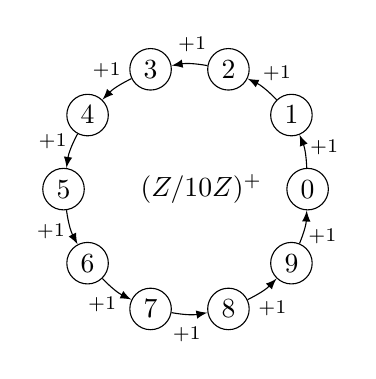
\begin{tikzpicture}[
        nd/.style={draw, circle, inner sep=0.2ex, minimum size=1.5em},
      ]
      \foreach \x [count=\i] in {36,72,...,324} {
        \node (v\i) at (\x:1.6) [nd] {$\i$};
      }
      \node (v0) at (0:1.5) [nd] {$0$};
      \foreach \x [count=\i from 2] in {3,4,...,9} {
        \pgfmathsetmacro\shang{10+36*\i}
        \path[-latex, draw] (v\i) edge[bend right=10] node[shift=(\shang:0.25)]{\scriptsize $+1$} (v\x);
      }
      \foreach \x/\i in {9/0,0/1,1/2} {
        \pgfmathsetmacro\shang{10+36*\x}
        \path[-latex, draw] (v\x) edge[bend right=10] node[shift=(\shang:0.25)]{\scriptsize $+1$} (v\i);
      }
      \node at (0.15, 0) {$(\mathbb{Z} / 10 \mathbb{Z})^+$};
    \end{tikzpicture}
    \quad
    \onslide<2->{
    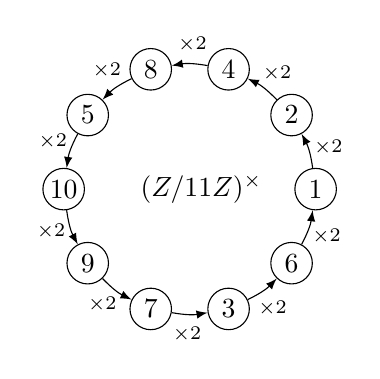
\begin{tikzpicture}[
        nd/.style={draw, circle, inner sep=0.2ex, minimum size=1.5em},
      ]
      \foreach \c/\x [count=\i from 0] in {
        1/0,
        2/36,
        4/72,
        8/108,
        5/144,
        10/180,
        9/216,
        7/252,
        3/288,
        6/324
      } {
        \node (v\i) at (\x:1.6) [nd] {$\c$};
      }
      \foreach \x [count=\i from 2] in {3,4,...,9} {
        \pgfmathsetmacro\shang{10+36*\i}
        \path[-latex, draw] (v\i) edge[bend right=10] node[shift=(\shang:0.25)]{\scriptsize $\times 2$} (v\x);
      }
      \foreach \x/\i in {9/0,0/1,1/2} {
        \pgfmathsetmacro\shang{10+36*\x}
        \path[-latex, draw] (v\x) edge[bend right=10] node[shift=(\shang:0.25)]{\scriptsize $\times 2$} (v\i);
      }
      \node at (0.15, 0) {$(\mathbb{Z} / 11 \mathbb{Z})^\times$};
    \end{tikzpicture}
    }
  \end{figure}
  \onslide<3-> {
    $\implies$ 模 $11$ 下的乘法等同於模 $10$ 下的加法。
  }
\end{frame}

\begin{frame}
  %\begin{definition}[階]
    %定義 $n \defeq \operatorname{ord}_m(a)$ 為最小的正整數 $n$ 使得 $a^n \equiv 1 \pmod{m}$。
  %\end{definition}
  %\pause

  \begin{definition}[原根]
    如果 $a^k$ 遍歴所有 $(\bZ / m \bZ)^\times$ 下的元素,我們就說 $a$ 是一個\emph{原根}。
  \end{definition}
  \pause

  \begin{theorem}[原根存在的條件]
    原根存在若且唯若 $m = 1, 2, 4, p^k, 2p^k$。
  \end{theorem}
  \pause
\end{frame}

\begin{frame}
  \begin{theorem}[Euler 定理]
    \begin{itemize}
      \item 對於質數 $p$,$a^{p-1} \equiv 1 \pmod{p}$。
      \item 對於任何數 $m$,$a^{\varphi(m)} \equiv 1 \pmod{m}$。
    \end{itemize}
  \end{theorem}
  \pause \disskip

  \[ a \cdot a^{\varphi(m) - 1} \equiv 1 \pmod{m} \implies a^{-1} \equiv a^{\varphi(m) - 1} \pmod{m} \]
\end{frame}

\begin{frame}
  \begin{problem}[An Easy Problem -- Subtask \#4, NTUJ 1423]
    給你 $b$, $c$, $p$,請你求 $a$ 使得 $a^b \equiv c \pmod{p}$。\\
    ($b, c, p \leq 10^9$, $p$ 是數且 $\gcd(b, p-1) \leq 10^5$)
  \end{problem} \pause

  請看講義…
\end{frame}
\end{document}
